%%%%%%%%%%%%%%%%%%%%%%%%%%%%%%%%%%%%%%%%%
% Beamer Presentation
% LaTeX Template
% Version 1.0 (10/11/12)
%
% This template has been downloaded from:
% http://www.LaTeXTemplates.com
%
% License:
% CC BY-NC-SA 3.0 (http://creativecommons.org/licenses/by-nc-sa/3.0/)
%
%%%%%%%%%%%%%%%%%%%%%%%%%%%%%%%%%%%%%%%%%

%----------------------------------------------------------------------------------------
% PACKAGES AND THEMES
%----------------------------------------------------------------------------------------

\documentclass[table, xcolor={dvipsnames}, 9pt]{beamer}
\usepackage{tikz}
\usetikzlibrary{positioning}
\mode<presentation> {

% The Beamer class comes with a number of default slide themes
% which change the colors and layouts of slides. Below this is a list
% of all the themes, uncomment each in turn to see what they look like.

%\usetheme{default}
%\usetheme{AnnArbor}
%\usetheme{Antibes}
%\usetheme{Bergen}
%\usetheme{Berkeley}
%\usetheme{Berlin}
%\usetheme{Boadilla}
%\usetheme{CambridgeUS}
%\usetheme{Copenhagen}
%\usetheme{Darmstadt}
%\usetheme{Dresden}
%\usetheme{Frankfurt}
%\usetheme{Goettingen}
%\usetheme{Hannover}
%\usetheme{Ilmenau}
%\usetheme{JuanLesPins}
%\usetheme{Luebeck}
% \usetheme{Madrid}
\usetheme{metropolis}
%\usetheme{Malmoe}
%\usetheme{Marburg}
%\usetheme{Montpellier}
%\usetheme{PaloAlto}
%\usetheme{Pittsburgh}
%\usetheme{Rochester}
%\usetheme{Singapore}
%\usetheme{Szeged}
%\usetheme{Warsaw}

% As well as themes, the Beamer class has a number of color themes
% for any slide theme. Uncomment each of these in turn to see how it
% changes the colors of your current slide theme.

%\usecolortheme{albatross}
%\usecolortheme{beaver}
%\usecolortheme{beetle}
%\usecolortheme{crane}
%\usecolortheme{dolphin}
%\usecolortheme{dove}
%\usecolortheme{fly}
%\usecolortheme{lily}
%\usecolortheme{orchid}
%\usecolortheme{rose}
%\usecolortheme{seagull}
%\usecolortheme{seahorse}
%\usecolortheme{whale}
%\usecolortheme{wolverine}

%\setbeamertemplate{footline} % To remove the footer line in all slides uncomment this line
%\setbeamertemplate{footline}[page number] % To replace the footer line in all slides with a simple slide count uncomment this line

%\setbeamertemplate{navigation symbols}{} % To remove the navigation symbols from the bottom of all slides uncomment this line
}

\usepackage{graphicx} % Allows including images
\usepackage{booktabs} % Allows the use of \toprule, \midrule and \bottomrule in tables
\usepackage{multirow}
\usepackage{natbib}
\usepackage[]{hyperref}
\usepackage{diagbox}
\usepackage{makecell}
\usepackage{subfig}
\usepackage{amsmath}
\usepackage{amsfonts,amsthm,amsmath,amssymb}    
\usepackage{bbm}
\usepackage{bm}
\usepackage{empheq}
\makeatletter
\let\save@measuring@true\measuring@true
\def\measuring@true{%
  \save@measuring@true
  \def\beamer@sortzero##1{\beamer@ifnextcharospec{\beamer@sortzeroread{##1}}{}}%
  \def\beamer@sortzeroread##1<##2>{}%
  \def\beamer@finalnospec{}%
}
\makeatother
\hypersetup{unicode=true,
            pdfusetitle,
            bookmarks=true,
            bookmarksnumbered=true,
            bookmarksopen=true,
            bookmarksopenlevel=2,
            breaklinks=false,
            pdfborder={0 0 1},
            backref=true,
            hypertexnames=false,
            pdfstartview={XYZ null null 1}}
\usepackage{xcolor}
\newcommand\myheading[1]{%
  \par\bigskip
  {\Large\bfseries#1}\par\smallskip}
\newcommand\given[1][]{\:#1\vert\:}
\theoremstyle{newstyle}
\newtheorem{thm}{Theorem}
\newtheorem{prop}[thm]{Proposition}
\newtheorem{lem}{Lemma}
\newtheorem{cor}{Corollary}
\newtheorem{defin}{Definition}
\newcommand*\diff{\mathop{}\!\mathrm{d}}
\newcommand*\Diff[1]{\mathop{}\!\mathrm{d^#1}}
\newcommand*{\QEDA}{\hfill\ensuremath{\blacksquare}}%
\newcommand*{\QEDB}{\hfill\ensuremath{\square}}%
\DeclareMathOperator{\E}{\mathrm{E}}
\DeclareMathOperator{\R}{\mathbb{R}}
\DeclareMathOperator{\Var}{\rm{Var}}
\DeclareMathOperator{\Cov}{\rm{Cov}}
\DeclareMathOperator{\e}{\rm{e}}
\DeclareMathOperator{\logit}{\rm{logit}}
\DeclareMathOperator{\indep}{{\perp\!\!\!\perp}}
%\DeclareMathOperator{\Pr}{\rm{Pr}}
\newenvironment{Column}[1][.5\linewidth]{\begin{column}{#1}}{\end{column}}
%----------------------------------------------------------------------------------------
% TITLE PAGE
%----------------------------------------------------------------------------------------

\title[]{Instrumental variables} % The short title appears at the bottom of every slide, the full title is only on the title page

\author{Thomas Leavitt} % Your name
\institute[] % Your institution as it will appear on the bottom of every slide, may be shorthand to save space
{
% Your institution for the title page
\medskip
\textit{} % Your email address
}
\date{\today} % Date, can be changed to a custom date

\begin{document}

\begin{frame}
\titlepage % Print the title page as the first slide
\end{frame}

%\begin{frame}
%\frametitle{Overview} % Table of contents slide, comment this block out to remove it
%\tableofcontents % Throughout your presentation, if you choose to use \section{} and \subsection{} commands, these will automatically be printed on this slide as an overview of your presentation
%\end{frame}

%------------------------------------------------------------------------
% PRESENTATION SLIDES
%------------------------------------------------------------------------
\section{Instrumental variable estimation}
\begin{frame}{Standard IV framework}
\begin{itemize}
\item As we did in the section on experiments, assume
\begin{enumerate}
\item \pause No-interference (each unit has only two potential outcomes)
\item \pause Random assignment of $Z$
\end{enumerate}	
\item \pause $\widehat{\text{ITT}}_Y$ is the Difference-in-Means estimator $\hat{\bar{\tau}}\left(\mathbf{Z}, \mathbf{Y}\right)$ 
\item \pause $\widehat{\text{ITT}}_D$ is the Difference-in-Means estimator $\hat{\bar{\tau}}\left(\mathbf{Z}, \mathbf{D}\right)$ 
\item \pause We know that 
\begin{itemize}
\item \pause $\E\left[\widehat{\text{ITT}}_Y\right] = \bar{\tau}_Y$ and 
\item \pause $\E\left[\widehat{\text{ITT}}_D\right] = \bar{\tau}_D = p_C - p_D$ (the proportion of Compliers minus the proportion of Defiers)
\end{itemize}
\item \pause Note that $\E\left[\cfrac{\widehat{\text{ITT}}_Y}{\widehat{\text{ITT}}_D}\right] \neq \cfrac{\E\left[\widehat{\text{ITT}}_Y\right]}{\E\left[\widehat{\text{ITT}}_D\right]}$, but ...
\begin{itemize}
\item \pause $\cfrac{\widehat{\text{ITT}}_Y}{\widehat{\text{ITT}}_D} \overset{p}{\to} \cfrac{\E\left[\widehat{\text{ITT}}_Y\right]}{\E\left[\widehat{\text{ITT}}_D\right]} = \cfrac{\bar{\tau}_Y}{\bar{\tau}_D}$
\end{itemize}
\end{itemize}
\end{frame}
%------------------------------------------------------------------------
\begin{frame}{IV estimator}
\begin{itemize}
\item With no additional assumptions, our IV (aka CACE, Bloom, Wald) estimator is consistent for the ratio of two average treatment effects, the average effect of (1) $Z$ on $Y$ and of (2) $Z$ on $D$
\item \pause However, we are often interested in the average causal effect of $D$ on $Y$
\begin{itemize}
\item \pause E.g., the effect of exercise on health, \textit{not} the effect of encouragement to exercise on health
\end{itemize}
\item \pause We will show under $3$ additional assumptions that $\cfrac{\bar{\tau}_Y}{\bar{\tau}_D}$ is equal to the average causal effect of $D$ on $Y$ for a \textit{subgroup} of the study population
\end{itemize}	
\end{frame}
%------------------------------------------------------------------------
\begin{frame}{IV estimator of CACE}
\begin{itemize}
\item Before we lay out the additional $3$ assumptions, first note that
\begin{itemize}
\item \pause $\bar{\tau}_Y = \delta_C p_C + \delta_{AT} p_{AT} + \delta_{NT} p_{NT} + \delta_D p_D$
\item \pause $\bar{\tau}_D = p_C - p_D$
\end{itemize}	
\item \pause $3$ more identification assumptions:
\begin{enumerate}
\item \pause \textbf{Exclusion restriction}: $Z$ affects $Y$ only through $D$
\begin{itemize}
\item \pause This means that $y_{Ti} = y_{Ci}$ for all $i: d_{Ti} = d_{Ci}$
\item \pause $\implies \delta_{AT} = 0 \text{ and }\delta_{NT} = 0$
\end{itemize}
\item \pause \textbf{No Defiers}: $p_D = 0$
\item \pause \textbf{Non-zero proportion of Compliers}: $p_C > 0$
\end{enumerate}	
\item \pause Under these three assumptions,
\begin{align*}
\cfrac{\bar{\tau}_Y}{\bar{\tau}_D} & = \cfrac{\delta_C p_C + \delta_{AT} p_{AT} + \delta_{NT} p_{NT} + \delta_D p_D}{p_C - p_D} \pause \\
& = \cfrac{\delta_C p_C + \delta_D p_D}{p_C - p_D} \pause \\
& = \cfrac{\delta_C p_C}{p_C} \pause \\
& = \delta_C
\end{align*} 
\item \pause Therefore, $\cfrac{\widehat{\text{ITT}}_Y}{\widehat{\text{ITT}}_D} \overset{p}{\to} \delta_C$
\end{itemize}
\end{frame}
%------------------------------------------------------------------------
\begin{frame}{Summary: IV estimator of CACE}
\begin{itemize}
\item Recall that under no-interference and random assignment, $\cfrac{\widehat{\text{ITT}}_Y}{\widehat{\text{ITT}}_D} \overset{p}{\to} \cfrac{\bar{\tau}_Y}{\bar{\tau}_D}$
\item \pause We then reexpressed $\cfrac{\bar{\tau}_Y}{\bar{\tau}_D}$ as $\cfrac{\bar{\tau}_Y = \delta_C p_C + \delta_{AT} p_{AT} + \delta_{NT} p_{NT} + \delta_D p_D}{p_C - p_D}$
\item \pause Then under (1) exclusion restriction, (2) no Defiers and (3) nonzero proportion of Compliers, we showed that 
\begin{align*}
\cfrac{\bar{\tau}_Y = \delta_C p_C + \delta_{AT} p_{AT} + \delta_{NT} p_{NT} + \delta_D p_D}{p_C - p_D} & = \delta_C
\end{align*}
\item \pause Therefore, it follows that $\cfrac{\widehat{\text{ITT}}_Y}{\widehat{\text{ITT}}_D} \overset{p}{\to} \delta_C$
\item \pause Intuitively, $\delta_C$ is the average of all Compliers' individual causal effects when $D = 1$ minus the average of all Compliers' individual causal effects when $D = 0$
\end{itemize}
\end{frame}
%------------------------------------------------------------------------
\section{Variance of IV estimator}
\begin{frame}{Variance of IV estimator}
\begin{itemize}
\item Recall that there exist analytic expressions for $\Var\left[\widehat{\text{ITT}}_Y\right]$ and $\Var\left[\widehat{\text{ITT}}_D\right]$
\item \pause We can conservatively estimate $\Var\left[\widehat{\text{ITT}}_Y\right]$ and $\Var\left[\widehat{\text{ITT}}_D\right]$ via $\widehat{\Var}\left[\widehat{\text{ITT}}_Y\right]$ and $\widehat{\Var}\left[\widehat{\text{ITT}}_D\right]$
\item \pause However, in general, there is no closed-form analytic expression for the variance of a random ratio
\item \pause We do not have an estimator for $\Var\left[\cfrac{\widehat{\text{ITT}}_Y}{\widehat{\text{ITT}}_D}\right]$ that is known to be unbiased, consistent or conservative
\item \pause Bloom (1984) proposed treating $\widehat{\text{ITT}}_D$ as fixed
\item \pause Others use Delta method (Taylor series approximation), e.g., in \texttt{AER} package in \texttt{R}
\end{itemize}	
\end{frame}
%------------------------------------------------------------------------
\section{Hypothesis Tests about Complier causal effects}
\begin{frame}{{Hypothesis Tests about Complier causal effects}}
\begin{itemize}
\item We can test the sharp null hypothesis no effect among all units
\item \pause We know by random assignment that
\begin{enumerate}
\item \pause this test will have a type I error probability at least as small as $\alpha$
\item \pause Will have power greater than $\alpha$ for a class of alternative hypotheses
\end{enumerate}
\item \pause Under what conditions is a test of the sharp null of no effect among all units equivalent to a test of the sharp null of no effect among Compliers?
\begin{enumerate}
\item \pause Exclusion restriction
\item \pause No Defiers
\item \pause Non-zero proportion of Compliers
\end{enumerate}	
\item \pause What about non-interference? For $Y$? For $D$?
\begin{itemize}
\item \pause Can we generalize exclusion restriction, no Defiers and nonzero proportion of Compliers under violations of interference?
\end{itemize}	
\end{itemize}	
\end{frame}
%------------------------------------------------------------------------
\begin{frame}{Sharp null hypothesis testing example}
\begin{itemize}
\item Imagine that our observed data is as follows: \pause 
\item[]
\item []\begin{table}[H]
\centering
    \begin{tabular}{l|l|l|l|l|l|l}
    $\mathbf{z}$ & $\mathbf{y}$ & $\mathbf{y_c}$ & $\mathbf{y_t}$ & $\mathbf{d}$ & $\mathbf{d_c}$ & $\mathbf{d_t}$ \\ \hline
    1 & 14 & ? & 14 & 0 & ? & 0 \\
    0 & 22 & 22 & ? & 0 & 0 & ? \\
    1 & 21 & ? & 21 & 1 & ? & 1 \\
    1 & 36 & ? & 36 & 1 & ? & 1 \\
    0 & 23 & 23 & ? & 0 & 0 & ? \\
    0 & 12 & 12 & ? & 1 & 1 & ? \\
    0 & 25 & 25 & ? & 1 & 1 & ? \\
    1 & 27 & ?  & 27 & 0 & ? & 0\\
    \end{tabular}
    \caption{Observed experimental data}
\end{table} \pause 
\item[]
\item The observed Difference-in-Means test statistic, $\hat{\bar{\tau}}\left(\mathbf{Z}, \mathbf{Y}\right)$, is $16.75$.  
\end{itemize}

\end{frame}
%------------------------------------------------------------------------
\begin{frame}{Sharp null hypothesis testing example}
\begin{itemize}
\item The sharp null hypothesis of no effect for all units:
\item[]
\item[]
\begin{table}[H]
\centering
    \begin{tabular}{l|l|l|l|l|l|l|l}
    $\mathbf{z}$ & $\mathbf{y}$ & $\mathbf{y_c}$ & $\mathbf{y_t}$ & $\mathbf{d}$ & $\mathbf{d_c}$ & $\mathbf{d_t}$ & Principal stratum\\ \hline
    1 & 14 & 14 & 14 & 0 & ? & 0 & Never Taker or Defier\\
    0 & 22 & 22 & 22 & 0 & 0 & ? & Complier or Never Taker\\
    1 & 21 & 21 & 21 & 1 & ? & 1 & Complier or Always Taker \\
    1 & 36 & 36 & 36 & 1 & ? & 1 & Complier or Always Taker \\
    0 & 23 & 23 & 23 & 0 & 0 & ? & Complier or Never Taker \\
    0 & 12 & 12 & 12 & 1 & 1 & ? & Always Taker or Defier \\
    0 & 25 & 25 & 25 & 1 & 1 & ? & Always Taker or Defier\\
    1 & 27 & 27  & 27 & 0 & ? & 0 & Never Taker or Defier \\
    \end{tabular}
    \caption{Sharp null of no effect for all units}
\end{table}  
\end{itemize}
\end{frame}
%------------------------------------------------------------------------
\begin{frame}{Sharp null hypothesis testing example}
\begin{itemize}
\item The null hypothesis of no effect among compliers under exclusion restriction, no Defiers and nonzero proportion of Compliers assumptions:
\item[]
\item[]
\begin{table}[H]
\centering
    \begin{tabular}{l|l|l|l|l|l|l|l}
    $\mathbf{z}$ & $\mathbf{y}$ & $\mathbf{y_c}$ & $\mathbf{y_t}$ & $\mathbf{d}$ & $\mathbf{d_c}$ & $\mathbf{d_t}$ & \text{Principal stratum}\\ \hline
    1 & 14 & 14 & 14 & 0 & 0 & 0 & Never Taker\\
    0 & 22 & 22 & 22 & 0 & 0 & ? & Complier or Never Taker \\
    1 & 21 & 21 & 21 & 1 & ? & 1 & Complier or Always Taker \\
    1 & 36 & 36 & 36 & 1 & ? & 1 & Complier or Always Taker \\
    0 & 23 & 23 & 23 & 0 & 0 & ? & Complier or Never Taker\\
    0 & 12 & 12 & 12 & 1 & 1 & 1 & Always Taker \\
    0 & 25 & 25 & 25 & 1 & 1 & 1 & Always Taker \\
    1 & 27 & 27  & 27 & 0 & 0 & 0 & Never Taker \\
    \end{tabular}
    \caption{Sharp null of no effect among Compliers}
    \label{tab: pot outs under null}
\end{table}   
\item[]
\item We don't need to know which of units 2  -- 5 are Compliers, only that at least one of these $4$ units is a Complier
\end{itemize}
\end{frame}
%------------------------------------------------------------------------
\begin{frame}{Sharp null hypothesis testing example}
\begin{itemize}
\item[]
\item[]	
\begin{figure}[H]
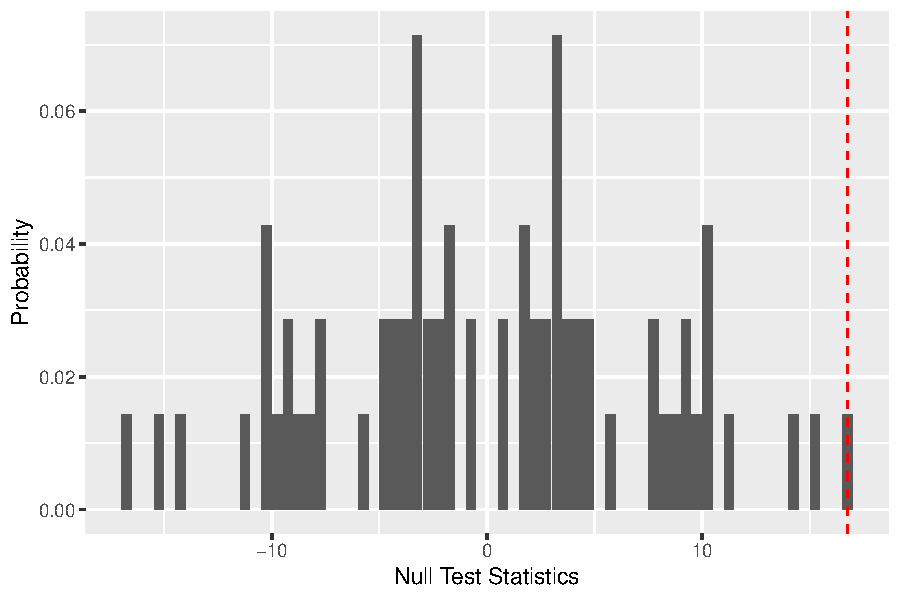
\includegraphics[width = \linewidth]{null_dist_plot.pdf}
\caption{Distribution of the Difference-in-Means test statistic under the sharp null of no effect}
\end{figure}
\end{itemize}
\end{frame}
%------------------------------------------------------------------------
\end{document}